\chapter[Clustering Uncertain Data Based on GLD Similarity]{Clustering Uncertain Data Based on GLD Similarity}\label{cap:gld_clustering}

\section{Related Works}

\cite{Jiang2011}

\section{Clustering Based on GLD}

Seudo codigo aqui con la explicacion de que es lo que pensamos hacer.

\begin{algorithm} 
\caption{Fitting the GLD to a spatio-temporal dataset}\label{alg:fitGLD}
\begin{algorithmic}[1] 
\Function{gldFit}{$S(s_{i},t_{j},<q_1,q_2,...,q_n>)$} 
\State $<\lambda_{1},\lambda_{2},\lambda_{3},\lambda_{4}> \gets \Call {fit.gld.lm}{<q_1,q_2,...,q_n>}$

\State $isValid_{(s_{i},t_{j})} \gets \Call {validityCheck}{<\lambda_{3},\lambda_{4}>}$
\If{$isValid_{(s_{i},t_{j})}$}
\State $[pvalue,D]_{(s_{i},t_{j})} \gets \Call{ks}{<\lambda_{1},\lambda_{2},\lambda_{3},\lambda_{4}>_{(s_{i},t_{j})}}$
\EndIf
\If{$pvalue_{(s_{i},t_{j})} > 0.05$}
\State $\Call{storeLambdas}{<\lambda_{1},\lambda_{2},\lambda_{3},\lambda_{4}>,s_{i},t_{j}}$
\EndIf
\EndFunction 
\end{algorithmic} 
\end{algorithm} 

\section{Empirical Study}

In this section we are going to test our hypothesis in two synthetic datasets. To generate those datasets we are going to use 4 different probabiltiy density functions: Gaussian, Exponential, Uniform and Gamma. The Gaussian distribution, equation \ref{eq:gaussian_distribution}

\begin{equation}\label{eq:gaussian_distribution}
f(x) = \frac{1}{{ \sqrt {2\pi \sigma} }}e^{{{ - \left( {x - \mu } \right)^2 } \mathord{\left/ {\vphantom {{ - \left( {x - \mu } \right)^2 } {2\sigma ^2 }}} \right. \kern-\nulldelimiterspace} {2\sigma ^2 }}}
\end{equation}

where:
\begin{itemize}
\item $\mu$ is the mean or expectation of the distribution (and also its median and mode),
\item $\sigma$ is the standard deviation, and
\item $\sigma^2$ is the variance.
\end{itemize}


\begin{equation}
  f(x) =
  \begin{cases}
    \lambda e^{-\lambda x} & \text{$x >= 0 $} \\
    0 & \text{$x < 0$}
  \end{cases}
\end{equation}

\begin{equation}
  f(x) =
  \begin{cases}
    \frac{1}{b-a} & \text{$a < x < b$} \\
    0 & \text{$x < a$ or $x > b$}
  \end{cases}
\end{equation}

\begin{equation}
  f(x) =
  \begin{cases}
    \frac{x^{\alpha-1}e^{\frac{-x}{\theta}}}{\Gamma(\alpha)\theta^{\alpha}} & \text{$x >= 0 $} \\
    0 & \text{$x < 0$}
  \end{cases}
\end{equation}

\section{Synthetic Data I}
To generate the first synthetic data set we use 11 probability density functions, where 5 are Gaussian, 5 Exponential, and one Uniform. The variance of the 5 Gaussian distributions is $0.05*i$, with $i=1, 2, 3, 4, 5$, and we generate 90 samples of each distribution. This is, the first 90 objects where generated from a Gaussian distribution with variance 0.05, and so on. Similarly, the rate of the 5 Exponential distributions is $0.05*i$, and again we generate 90 samples of each one. Finally, 100 samples of a Uniform distribution between $[0, 1]$ were generated. In resume, we have 1000 objects, where the first 450 were sampled from Gaussian distributions, the next 450 from an Exponential and the last 100 from a Uniform distribution. As we generate a synthetic dataset in this way, we have the ground truth of the clustering in the dataset. This ground truth is used to evaluate the clustering quality of our algorithms.

\subsection{Clustering using $\lambda_{2}$, $\lambda_{3}$ and $\lambda_{4}$}

Clusters que formaron la imagen normal exponencial uniform2
cl clusters size
   86  86 100  93  90 195 102  84   5  90  69
 
Clusters que formaron la imagen normal exponencial uniform3 
 cl clusters size
   82  93   5 198 102  83  91  82  90  84  90

\begin{figure}[H]
    \centering
    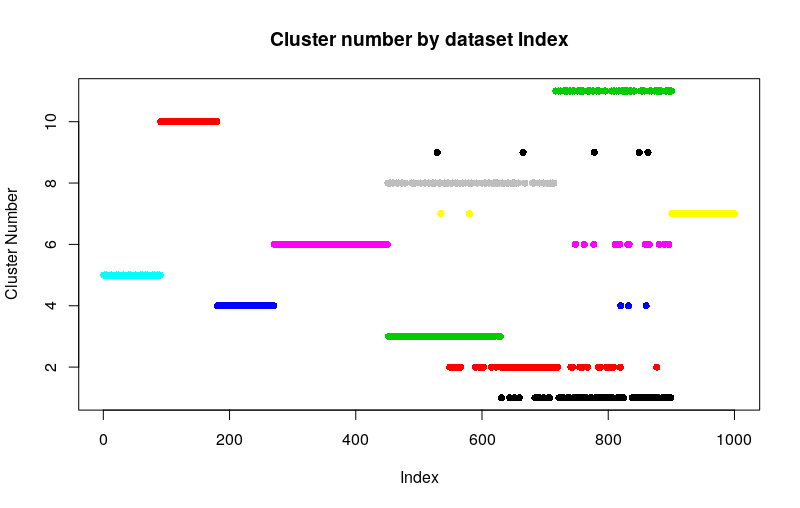
\includegraphics[width=0.8\textwidth]{img/gld_clustering/Dataset1/l2_l3_l4/normal_exponential_uniform2.png}
    \caption{Goodness of the fit based on the \textit{p}-value}
    \label{fig:p_value}
\end{figure}

\subsection{Clustering using $\lambda_{3}$ and $\lambda_{4}$}

 cl1 clusters size
  197 118 110  35  41  65   2 131  74 105 122
 

\subsection{Effectiveness of the Clustering}

\section{Synthetic Data II}

\subsection{Clustering using $\lambda_{2}$, $\lambda_{3}$ and $\lambda_{4}$}
cl2 clusters size
  100 106  91  20  67  89  90   6  26  52  92  95  73  90  90 363

\subsection{Clustering using $\lambda_{3}$ and $\lambda_{4}$}

\subsection{Effectiveness of the Clustering}

\section{Conclusions}